% --- IMPORTS ---
\documentclass[leqno]{article}
\usepackage{graphicx}
\usepackage{dsfont}
\usepackage{mathtools}
\usepackage{amssymb}
\usepackage{amsmath}
\usepackage{amsthm}
\usepackage{float}
\usepackage{ragged2e}
\usepackage{tensor}
\usepackage{fancyhdr}
\usepackage{empheq}
\usepackage[most]{tcolorbox}
\usepackage{enumitem}
\usepackage{dirtytalk}
\usepackage{marginnote}
\usepackage{microtype}
\usepackage[
  a4paper,
  left=0.8in,
  right=1in,
  top=1in,
  bottom=0.5in,
  headheight=14pt,
  headsep=0.4in
]{geometry}
\setlength{\parindent}{0cm}
% --- TikZ Packages ---
\usepackage{pgfplots}
\pgfplotsset{compat=1.18}
\usepgfplotslibrary{fillbetween, polar}
\usetikzlibrary{calc, positioning}
\usetikzlibrary{angles, quotes}
\usetikzlibrary{arrows.meta}
\usetikzlibrary{decorations.pathreplacing, decorations.markings}
\usetikzlibrary{patterns}
\usetikzlibrary{intersections}
% --- URL Packages ---
\usepackage[colorlinks=true,linkcolor=red,citecolor=magenta,urlcolor=black]{hyperref}%
\urlstyle{same}
% --- END OF IMPORTS ---

% --- CUSTOM COMMANDS ---
\RenewDocumentCommand{\marks}{o m}{%
  \IfValueTF{#1}%
    {\marginnote{\raggedright\textbf{[#2]}}[#1]}%
    {\marginnote{\raggedright\textbf{[#2]}}}%
}
\newcommand{\vspacerule}[2]{%
  \par\vspace*{#1}%
  \noindent\hrulefill\par
  \vspace*{#2}%
}
\definecolor{scarlet}{RGB}{205, 40, 75}
\newcommand{\questionitem}{%
  \item\phantomsection
  \addcontentsline{toc}{section}{Question \number\value{enumi}}%
}
\renewcommand{\contentsname}{Questions}
% --- END OF CUSTOM COMMANDS ---

% --- HEADER CONFIG ---
\pagestyle{fancy}
\fancyhead{}
\fancyfoot{}
\renewcommand{\headrulewidth}{0.9pt}
\lhead{Volumes of Revolution}
\chead{}
\rhead{\href{https://danieljsmith.org}{danieljsmith.org}}
% --- END OF HEADER CONFIG ---

\begin{document}
\vspace*{20pt}
\tableofcontents
\newpage
\begin{enumerate}[
  label=\textbf{\arabic*.},
  leftmargin=*,
  topsep=0pt,
  partopsep=0pt,
  parsep=0pt
]

% ---- Question 1 ----
\questionitem
% [Source: _QBT__Volumes_of_Revolution, Q1]

\begin{figure}[H]
    \centering
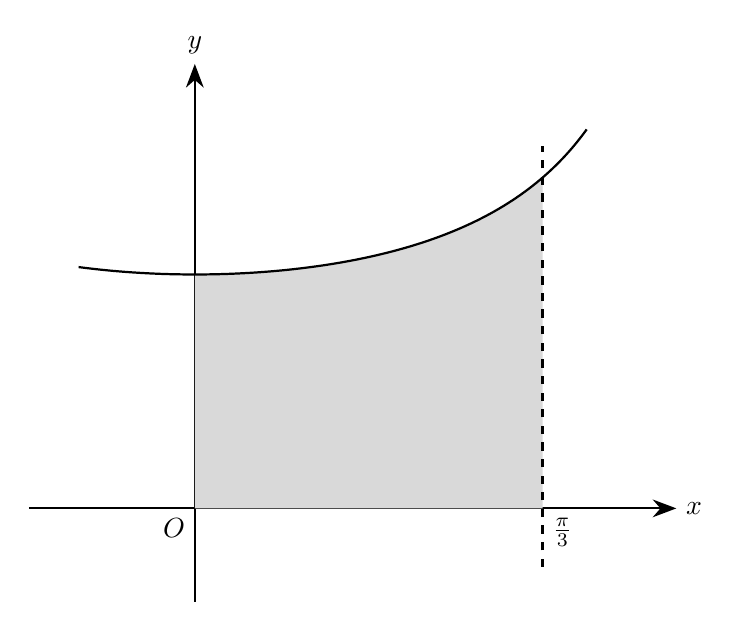
\begin{tikzpicture}[scale=1.2]
\def\xa{1.0472}
\begin{axis}[
    axis lines=middle,
    axis line style={-{Stealth[length=3mm]}, thick, black},
    xlabel={$x$},
    ylabel={$y$},
    xmin=-0.5, xmax=1.45,
    ymin=-0.4, ymax=1.9,
    xtick=\empty,
    ytick=\empty,
    clip=false,
    every axis x label/.style={at={(ticklabel* cs:1)}, anchor=west},
    every axis y label/.style={at={(ticklabel* cs:1)}, anchor=south}
]
\addplot[name path=curve, thick, black, samples=200, domain=-0.35:1.18] {sqrt(1/cos(deg(x)))};
\addplot[name path=xaxisline, draw=none, domain=0:\xa] {0};
\addplot[gray!30, draw=none] fill between[of=curve and xaxisline, soft clip={domain=0:\xa}];
\addplot[dashed, thick, black] coordinates {(\xa,-0.25) (\xa,1.55)};
\node[below left] at (axis cs:0,0) {$O$};
\node[below right] at (axis cs:\xa,0) {$\frac{\pi}{3}$};
\end{axis}
\end{tikzpicture}
\end{figure}


The shaded region is enclosed by the curve $y = \sqrt{\sec x}$, the coordinate axes and the line $x = \frac{\pi}{3}$. \\

The region is rotated completely about the $x$-axis. \\
Find the exact volume of the solid generated. \marks{3}

\newpage

% ---- Question 2 ----
\questionitem
% [Source: _QBT__Volumes_of_Revolution, Q2]

\begin{figure}[H]
    \centering
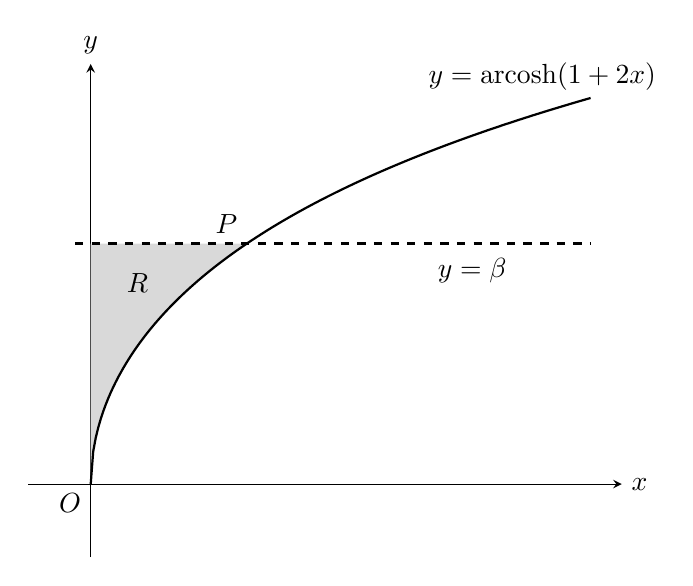
\begin{tikzpicture}[scale=1.1]
\pgfmathsetmacro{\betaval}{ln(2+sqrt(3))}
\pgfmathsetmacro{\alphaval}{1/2}
\begin{axis}[
    axis lines=center,
    xlabel={$x$},
    ylabel={$y$},
    xmin=-0.2, xmax=1.7,
    ymin=-0.4, ymax=2.3,
    xtick=\empty,
    ytick=\empty,
    clip=false,
    every axis x label/.style={at={(ticklabel* cs:1)}, anchor=west},
    every axis y label/.style={at={(ticklabel* cs:1)}, anchor=south},
]
\addplot[name path=lineclip, draw=none, domain=0:\alphaval] {\betaval};
\addplot[name path=curveclip, draw=none, samples=200, domain=0:\alphaval] {ln(1 + 2*x + sqrt((1 + 2*x)^2 - 1))};
\addplot[gray!30] fill between[of=lineclip and curveclip];
\addplot[thick, black, samples=200, domain=0:1.6] {ln(1 + 2*x + sqrt((1 + 2*x)^2 - 1))};
\addplot[thick, black, dashed, domain=-0.05:1.6] {\betaval};
\node[above right] at (axis cs:1.05,2.1) {$y=\operatorname{arcosh}(1+2x)$};
\node[right] at (axis cs:1.08,\betaval-0.15) {$y=\beta$};
\node at (axis cs:0.15,1.1) {$R$};
\node[below left] at (axis cs:0,0) {$O$};
\node[above left] at (axis cs:\alphaval,\betaval) {$P$};
\end{axis}
\end{tikzpicture}
\end{figure}


The diagram above shows a sketch of part of the curve with equation
\[
y = \operatorname{arcosh}(1 + 2x) \qquad x \geq 0
\] \\
and the straight line with equation $y = \beta$. \\

The line and the curve intersect at the point with coordinates $(\alpha, \beta)$. \\

Given that $\beta = \ln(2+\sqrt{3})$, \\

\begin{enumerate}[label=\textbf{(\alph*)}]
  \item show that $\alpha = \dfrac{1}{2}$. \marks{3} \\
\end{enumerate}
The finite region $R$, shown shaded in the diagram above, is bounded by the curve with equation $y = \operatorname{arcosh}(1 + 2x)$, the $y$-axis and the line with equation $y = \beta$. \\

  The region $R$ is rotated through $2\pi$ radians about the $y$-axis. \\
\begin{enumerate}[label=\textbf{(\alph*)}, resume]
\item Use calculus to find the exact value of the volume of the solid generated. \marks{6} \\
\end{enumerate}

\newpage


% ---- Question 3 ----
\questionitem
% [Source: _QBT__Volumes_of_Revolution, Q3]

The equation of a curve is
\[
y = \sqrt{\frac{k-x}{k+x}}
\]
where $k$ is a positive constant. The region enclosed by the curve, the $x$-axis, the $y$-axis and the line $x = k$ is rotated through $2\pi$ radians about the $x$-axis. \\

Given that the volume of the solid of revolution formed is $1$ unit$^3$, find the exact value of $k$. \marks{4}


\newpage


% ---- Question 4 ----
\questionitem
% [Source: _QBT__Volumes_of_Revolution, Q4]

\begin{enumerate}[label=\textbf{(\alph*)}]
  \item Find
  \[
  \int \sin^2\theta\,\mathrm{d}\theta
  \]
  \marks[-20pt]{2}
\end{enumerate}

\begin{figure}[H]
    \centering
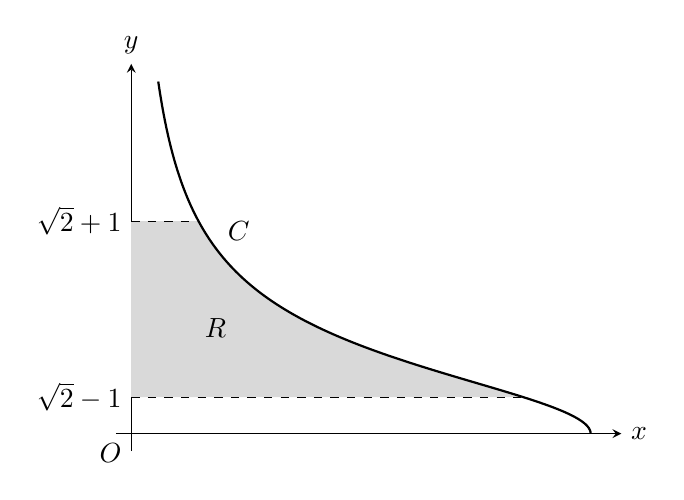
\begin{tikzpicture}
\pgfmathsetmacro{\ya}{sqrt(2)-1}
\pgfmathsetmacro{\yb}{sqrt(2)+1}
\pgfmathsetmacro{\xa}{6/(1+\ya*\ya)}
\pgfmathsetmacro{\xb}{6/(1+\yb*\yb)}
\begin{axis}[
    axis lines=center,
    xlabel={$x$},
    ylabel={$y$},
    xmin=-0.2, xmax=6.4,
    ymin=-0.2, ymax=4.2,
    xtick=\empty,
    ytick=\empty,
    width=8cm,
    height=6.5cm,
    clip=false,
    every axis x label/.style={at={(ticklabel* cs:1)}, anchor=west},
    every axis y label/.style={at={(ticklabel* cs:1)}, anchor=south}
]

\path[fill=gray!30]
    (axis cs:0,\ya) --
    (axis cs:0,\yb) --
    plot[domain=\yb:\ya, samples=200, variable=\u]
        (axis cs:{6/(1+\u^2)},{\u})
    -- cycle;

\addplot[thick, black, samples=200, domain=0:4, variable=\u]
    ({6/(1+\u^2)}, {\u})
    node[pos=0.72, above right] {$C$};

\addplot[dashed, black] coordinates {(0,\ya) (\xa,\ya)};
\addplot[dashed, black] coordinates {(0,\yb) (\xb,\yb)};

\node[below left] at (axis cs:0,0) {$O$};
\node[left] at (axis cs:0,\ya) {$\sqrt{2}-1$};
\node[left] at (axis cs:0,\yb) {$\sqrt{2}+1$};
\node at (axis cs:1.1,1.2) {$R$};

\end{axis}
\end{tikzpicture}
\end{figure}


The diagram shows part of the curve $C$ with parametric equations $x=6\sin^2\theta$, $y=\cot\theta$, $0<\theta\leq\frac{\pi}{2}$. \\

The finite region $R$ shown in the diagram is bounded by $C$, the lines $y=\sqrt{2}-1$, $y=\sqrt{2}+1$ and the $y$-axis. Region $R$ is rotated through $2\pi$ radians about the $y$-axis to form a solid of revolution. \\
\begin{enumerate}[label=\textbf{(\alph*)}, resume]
  \item Show that the volume of the solid of revolution formed is given by the integral
  \[
  k\int_a^b \sin^2\theta\,\mathrm{d}\theta
  \]
  where $a$, $b$ and $k$ are constants to be found. \marks{5} \\


\item Hence find the exact value of this volume, giving your answer in the form $p\pi^2$, where $p$ is a constant to be found. \marks{3} \\
\end{enumerate}

\newpage

% ---- Question 5 ----
\questionitem
% [Source: _QBT__Volumes_of_Revolution, Q5]

\begin{enumerate}[label=\textbf{(\alph*)}]
  \item Show that $\sinh(2\ln 2)=\frac{15}{8}$. \marks{2} \\
\end{enumerate}

\begin{figure}[H]
    \centering
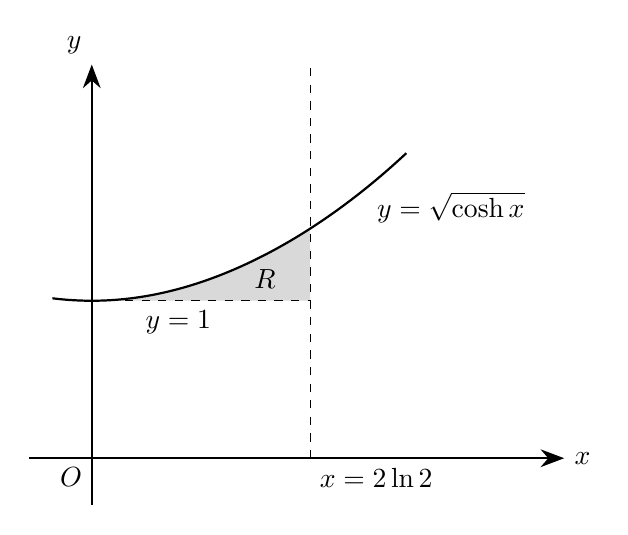
\begin{tikzpicture}[scale=2]
\def\xmin{-0.4}
\def\xmax{3}
\def\ymin{-0.3}
\def\ymax{2.5}
\def\xv{1.386294361}

\draw[-{Stealth[length=3mm]}, thick] (\xmin,0) -- (\xmax,0) node[right] {$x$};
\draw[-{Stealth[length=3mm]}, thick] (0,\ymin) -- (0,\ymax) node[above left] {$y$};

\fill[gray!30] (0,1) --
  plot[domain=0:\xv, samples=200] (\x, {sqrt((exp(\x)+exp(-\x))/2)}) --
  (\xv,1) -- cycle;

\draw[thick, domain=-0.25:2.0, samples=200] plot (\x, {sqrt((exp(\x)+exp(-\x))/2)});
\draw[dashed] (0,1) -- (\xv,1);
\draw[dashed] (\xv,0) -- (\xv,\ymax);

\node[below left] at (0,0) {$O$};
\node at (1.1,1.14) {$R$};
\node[above right] at (1.75,1.43) {$y=\sqrt{\cosh x}$};
\node[below right] at (0.28,1) {$y=1$};
\node[below right] at (\xv,0) {$x=2\ln 2$};
\end{tikzpicture}
\end{figure}


The region $R$ is bounded by the curve with equation $y=\sqrt{\cosh x}$, the line $y=1$ and the line $x=2\ln 2$, as shown in the diagram. The units of the axes are centimetres. \\

A designer models a hollow glass ornament as the solid formed by rotating $R$ completely about the $x$-axis. \\
\begin{enumerate}[label=\textbf{(\alph*)}, resume]
  \item Determine, according to the model, the exact volume of the ornament. \marks{4} \\
\end{enumerate}

\newpage

% ---- Question 6 ----
\questionitem
% [Source: _QBT__Volumes_of_Revolution, Q6]

\begin{figure}[H]
    \centering
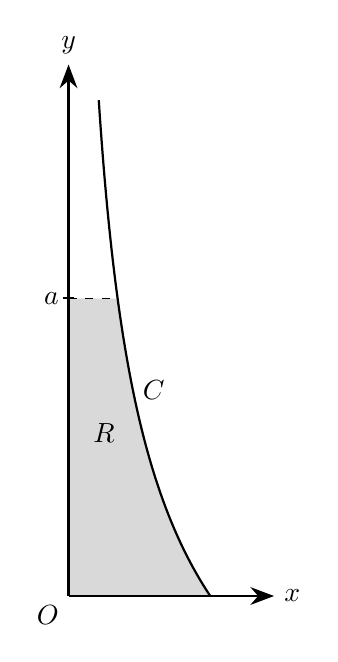
\begin{tikzpicture}[scale=1.8]
\def\a{2.1}
\def\ytop{3.5}
\def\xmax{1.45}
\def\ymax{3.75}
    \pgfmathsetmacro{\bx}{9/((\a+3)^2)}
\coordinate (O) at (0,0);
\coordinate (A) at (0,\a);
\coordinate (B) at (\bx,\a);
\coordinate (X) at (1,0);
\coordinate (RLab) at (0.25,1.15);
\coordinate (CLab) at ({9/((1.45+3)^2)},1.45);

\fill[gray!30] (O) -- (X) --
  plot[domain=0:\a, samples=200, variable=\yy] ({9/((\yy+3)^2)}, {\yy})
  -- (A) -- cycle;

\draw[thick, -{Stealth[length=3mm]}] (0,0) -- (\xmax,0) node[right] {$x$};
\draw[thick, -{Stealth[length=3mm]}] (0,0) -- (0,\ymax) node[above] {$y$};

\draw[thick] plot[domain=0:\ytop, samples=200, variable=\yy] ({9/((\yy+3)^2)}, {\yy});
\draw[dashed] (A) -- (B);

\draw[thick] (-0.04,\a) -- (0.04,\a);
\node[left] at (0,\a) {$a$};

\node[below left] at (O) {$O$};
\node at (RLab) {$R$};
\node[right] at (CLab) {$C$};
\end{tikzpicture}
\end{figure}


The curve $C$ is given parametrically by
\[
x = \frac{9}{t^4}, \qquad y = t^2 - 3, \qquad t \geq \sqrt{3}
\]
The shaded region $R$, shown in the diagram, is enclosed by $C$, the $x$-axis, the $y$-axis and the line $y=a$. When $R$ is rotated through $2\pi$ radians about the $y$-axis, the resulting solid has volume
\[
\frac{7\pi}{8}
\]
Find the exact value of $a$. \marks{8}

\newpage

% ---- Question 7 ----
\questionitem
% [Source: _QBT__Volumes_of_Revolution, Q7]

\begin{figure}[H]
    \centering
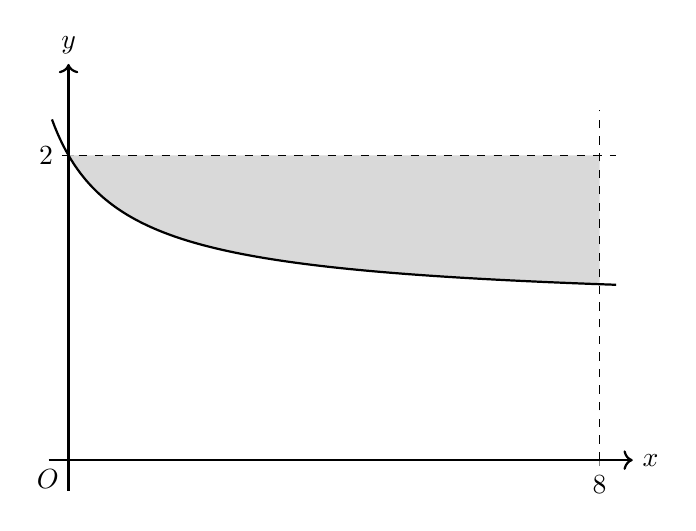
\begin{tikzpicture}
\begin{axis}[
    axis lines=middle,
    axis line style={->, thick},
    xlabel={$x$},
    ylabel={$y$},
    xmin=-0.3, xmax=8.5,
    ymin=-0.2, ymax=2.6,
    xtick={8},
    ytick={2},
    xticklabels={$8$},
    yticklabels={$2$},
    width=9cm,
    height=7cm,
    clip=false,
    every axis x label/.style={at={(ticklabel* cs:1)}, anchor=west},
    every axis y label/.style={at={(ticklabel* cs:1)}, anchor=south}
]
\addplot[name path=top, draw=none, domain=0:8, samples=2] {2};
\addplot[name path=curvefill, draw=none, domain=0:8, samples=200] {sqrt((x+4)/(x+1))};
\addplot[gray!30] fill between[of=top and curvefill];

\addplot[thick, black, domain=-0.25:8.25, samples=200] {sqrt((x+4)/(x+1))};
\addplot[dashed, black, domain=-0.1:8.25, samples=2] {2};
\addplot[dashed, black] coordinates {(8,0) (8,2.3)};

\node[below left] at (axis cs:0,0) {$O$};
\end{axis}
\end{tikzpicture}
\end{figure}


The diagram shows the region bounded by the curve $y = \sqrt{\dfrac{x+4}{x+1}}$, the line $y = 2$ and the line $x = 8$. The curve meets the line $y = 2$ at the point $(0,2)$. \\

Find the exact volume of the solid formed when this region is rotated through $360^\circ$ about the $x$-axis. \marks{6}

\newpage

% ---- Question 8 ----
\questionitem
% [Source: _QBT__Volumes_of_Revolution, Q8]

The region in the first quadrant bounded by the curve $y = \sinh x$, the $y$-axis, and the line $y = 2$ is rotated through $360^\circ$ about the $x$-axis. \\

Find the exact volume of revolution generated, expressing your answer in a form involving a logarithm. \marks{7}

\newpage


% ---- Question 9 ----
\questionitem
% [Source: _QBT__Volumes_of_Revolution, Q9]

\begin{figure}[H]
    \centering
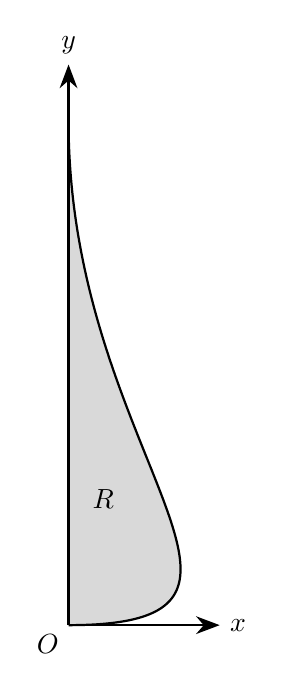
\begin{tikzpicture}[scale=0.8]
\def\tmax{1}
\def\xmax{2.4}
\def\ymax{8.9}

\fill[gray!30] (0,0)
  plot[samples=200,domain=0:\tmax,smooth,variable=\t] ({12*\t*(1-\t)*(1-\t)},{8*\t*\t}) -- cycle;

\draw[thick,-{Stealth[length=3mm]}] (0,0) -- (\xmax,0) node[right] {$x$};
\draw[thick,-{Stealth[length=3mm]}] (0,0) -- (0,\ymax) node[above] {$y$};
\draw[thick,samples=200,domain=0:\tmax,smooth,variable=\t] plot ({12*\t*(1-\t)*(1-\t)},{8*\t*\t});

\node[below left] at (0,0) {$O$};
\node at (0.55,2) {$R$};
\end{tikzpicture}
\end{figure}


Part of the side profile of a solid wooden ornament is shown in the diagram. \\
The outline is modelled by the curve with parametric equations
\[
x=12t(1-t)^2,\quad y=8t^2,\qquad 0 \le t \le 1
\] \\
The ornament is formed by rotating the shaded region through $2\pi$ radians about the $y$-axis. \\

Use the model to find the volume of the ornament. \marks{7}
\newpage

% ---- Question 10 ----
\questionitem
% [Source: _QBT__Volumes_of_Revolution, Q10]

\begin{figure}[H]
    \centering
\begin{tikzpicture}[x=3.0cm,y=1.2cm, scale=2]
\def\yTop{1.095}
\def\yBot{-1.08824}
\def\xLeft{-0.8}
\def\xRight{0.85}
\def\yMin{-1.3}
\def\yMax{1.3}

\coordinate (O) at (0,0);
\coordinate (TopI) at (0,\yTop);
\coordinate (BotI) at (0,\yBot);

\draw[-{Stealth[length=3mm]}, thick] (\xLeft,0) -- (\xRight,0) node[right] {$x$};
\draw[-{Stealth[length=3mm]}, thick] (0,\yMin) -- (0,\yMax) node[above] {$y$};

\draw[thick, smooth, variable=\yv, domain=\yBot:\yTop, samples=300]
  plot ({sqrt(max(0,(8 - 6*(\yv)*(\yv) - (\yv)*sin(deg(2*(\yv))))/20))}, {\yv});

\node[below left] at (O) {$O$};
\node[left] at (TopI) {$1.088$};
\node[left] at (BotI) {$-1.088$};
\end{tikzpicture}
\end{figure}


A chocolatier makes hand-rolled chocolate drops. \\

The tallest drop in one tray was approximately $2.2\,\mathrm{cm}$ high. \\

The shape of this drop is modelled by rotating the curve with equation
\[
20x^2 + 6y^2 + y\sin(2y) = 8, \qquad x \geq 0
\]
shown in the diagram above, about the $y$-axis through $2\pi$ radians, where the units are cm. \\

Given that the $y$-intercepts of the curve are $-1.088$ and $1.088$ to four significant figures, \\

\begin{enumerate}[label=\textbf{(\alph*)}]
  \item Use algebraic integration to determine, according to the model, the volume of this chocolate drop. \marks{6} \\
\end{enumerate}
The chocolatier melts down $80$ chocolate drops from the same tray. \\
\begin{enumerate}[label=\textbf{(\alph*)}, resume]
  \item Use your answer to part (a) to decide whether, in reality, there is likely to be enough chocolate to fill a mould of volume $140\,\mathrm{cm}^3$, giving a reason. \marks{2} \\
\end{enumerate}

\newpage

% ---- Question 11 ----
\questionitem
% [Source: _QBT__Volumes_of_Revolution, Q11]

\begin{figure}[H]
    \centering
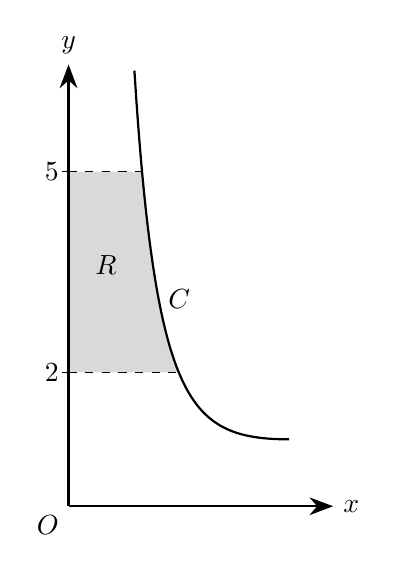
\begin{tikzpicture}[x=1.4cm,y=0.85cm]
\def\ylo{2}
\def\yhi{5}
\def\paramlo{1}
\def\paramhi{2}
\def\xmax{2.4}
\def\ymax{6.6}
\pgfmathsetmacro{\xlo}{2/(1+\paramlo)}
\pgfmathsetmacro{\xhi}{2/(1+\paramhi)}

\fill[gray!30] (0,\ylo) -- (0,\yhi) --
  plot[domain=\paramhi:\paramlo, samples=200, variable=\param] ({2/(1+\param)}, {\param*\param+1}) -- cycle;

\draw[thick, -{Stealth[length=3mm]}] (0,0) -- (\xmax,0) node[right] {$x$};
\draw[thick, -{Stealth[length=3mm]}] (0,0) -- (0,\ymax) node[above] {$y$};

\draw[dashed] (0,\ylo) -- (\xlo,\ylo);
\draw[dashed] (0,\yhi) -- (\xhi,\yhi);

\draw[thick, domain=0:2.35, samples=200, variable=\param]
  plot ({2/(1+\param)}, {\param*\param+1});

\draw (-0.06,\ylo) -- (0.06,\ylo);
\draw (-0.06,\yhi) -- (0.06,\yhi);
\node[left] at (0,\ylo) {$2$};
\node[left] at (0,\yhi) {$5$};
\node[below left] at (0,0) {$O$};

\node at (0.34,3.6) {$R$};
\coordinate (Pc) at ({2/(1+1.45)}, {1.45*1.45+1});
\node[right] at (Pc) {$C$};
\end{tikzpicture}
\end{figure}


The diagram shows part of the curve $C$ with parametric equations \[x=\frac{2}{1+t},\quad y=t^2+1,\qquad t\geq 0\] 

The region $R$ is bounded by the curve, the $y$-axis and the lines $y=2$ and $y=5$. Region $R$ is rotated through $2\pi$ radians about the $y$-axis. \\

Use parametric integration to find the volume of the resulting solid of revolution. \marks{6} \\

\newpage

% ---- Question 12 ----
\questionitem
% [Source: _QBT__Volumes_of_Revolution, Q12]

\begin{figure}[H]
    \centering
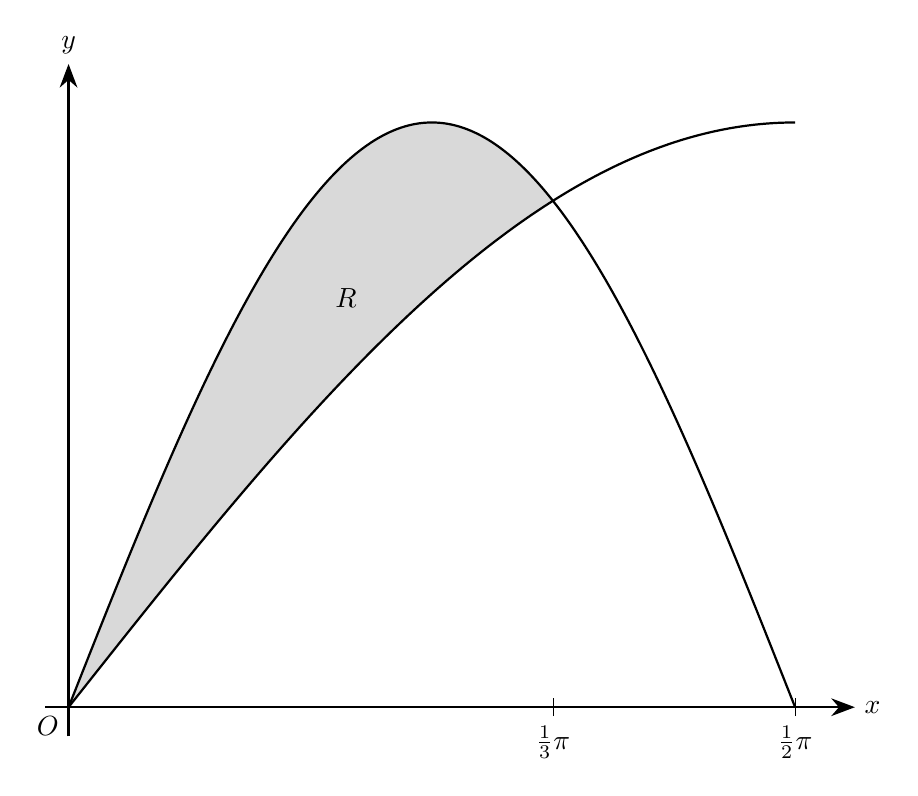
\begin{tikzpicture}[scale=1.5]
\def\halfpi{1.57079632679}
\def\thirdpi{1.04719755120}
\begin{axis}[
    axis lines=center,
    xlabel={$x$},
    ylabel={$y$},
    xmin=-0.05, xmax=1.7,
    ymin=-0.05, ymax=1.1,
    xtick={\thirdpi,\halfpi},
    xticklabels={$\frac{1}{3}\pi$,$\frac{1}{2}\pi$},
    ytick=\empty,
    clip=false,
    enlargelimits=false,
    axis line style={thick, black, -{Stealth[length=3mm]}},
    tick style={black},
    every axis x label/.style={at={(ticklabel* cs:1)}, anchor=west},
    every axis y label/.style={at={(ticklabel* cs:1)}, anchor=south}
]
\addplot[name path=sinx, thick, black, samples=200, domain=0:\halfpi] {sin(deg(x))};
\addplot[name path=sin2x, thick, black, samples=200, domain=0:\halfpi] {sin(deg(2*x))};
\addplot[gray!30] fill between[of=sin2x and sinx, soft clip={domain=0:\thirdpi}];
\node[below left] at (axis cs:0,0) {$O$};
\node at (axis cs:0.6,0.7) {$R$};
\end{axis}
\end{tikzpicture}
\end{figure}


The diagram shows the curves $y = \sin x$ and $y = \sin 2x$, for $0 \leq x \leq \frac{1}{2}\pi$. The shaded region $R$ is the finite region enclosed by the curves. \\

Find the volume of the solid of revolution formed when $R$ is rotated completely about the $x$-axis, giving your answer in terms of $\pi$. \marks{7} \\


\newpage

% ---- Question 13 ----
\questionitem
% [Source: _QBT__Volumes_of_Revolution, Q13]

\begin{figure}[H]
    \centering
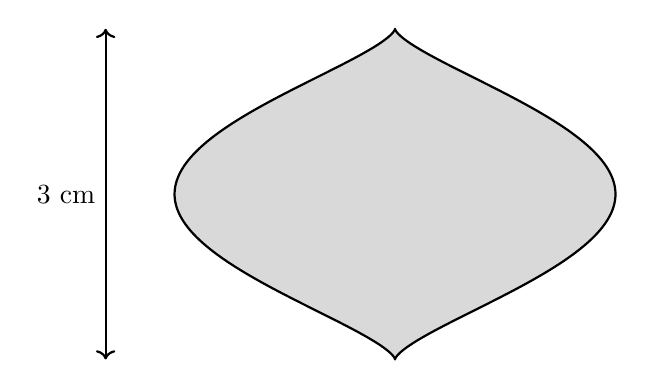
\begin{tikzpicture}[scale=2.1]
\def\dimx{-1.75}
\draw[thick, fill=gray!30, line join=round]
  plot[domain=0:360, samples=400, variable=\t]
    ({sin(\t) - (1/3)*sin(3*\t)}, {1 - cos(\t)})
  -- cycle;
\draw[<->, thick] (\dimx, 0) -- (\dimx, 2)
  node[midway, left] {$3\ \mathrm{cm}$};
\end{tikzpicture}
\end{figure}


The diagram shows the outline of a glass bead. The bead is modelled by the solid obtained when the region enclosed by a curve $C$ is rotated about the $y$-axis. The actual bead has height $3\ \mathrm{cm}$. The curve $C$ has parametric equations
\[
x = \sin\theta - \frac{1}{3}\sin 3\theta,\qquad y = 1 - \cos\theta,\qquad 0 \le \theta \le 2\pi
\] \\

\begin{enumerate}[label=\textbf{(\alph*)}]
  \item Show that a Cartesian equation of the curve $C$ is
  \[
  x^2 = \frac{16}{9}y^3(2-y)^3
  \]
  \marks[-20pt]{4}
  \item Hence, using the model, find, in $\mathrm{cm}^3$, the volume of the bead. \marks{5} \\
\end{enumerate}
\newpage
% ---- Question 14 ----
\questionitem
% [Source: _QBT__Volumes_of_Revolution, Q14]

The equation of a curve is \[y=\frac{x}{\sqrt{k^2+x^2}}\] where $k$ is a positive constant. \\

The region in the first quadrant bounded by the curve, the $x$-axis, the $y$-axis and the line $x=k$ is rotated through $2\pi$ radians about the $x$-axis

Given that the volume of revolution formed is $1\text{ unit}^3$, find the exact value of $k$ \marks{4} \

\newpage
% ---- Question 15 ----
\questionitem
% [Source: _QBT__Volumes_of_Revolution, Q15]

\begin{enumerate}[label=\textbf{(\alph*)}]
  \item Prove that
  \[
  \cos 4\theta \cos \theta \equiv \frac{1}{2}(\cos 5\theta + \cos 3\theta)
  \]
  \marks[-20pt]{3}
\end{enumerate}

\begin{figure}[H]
    \centering
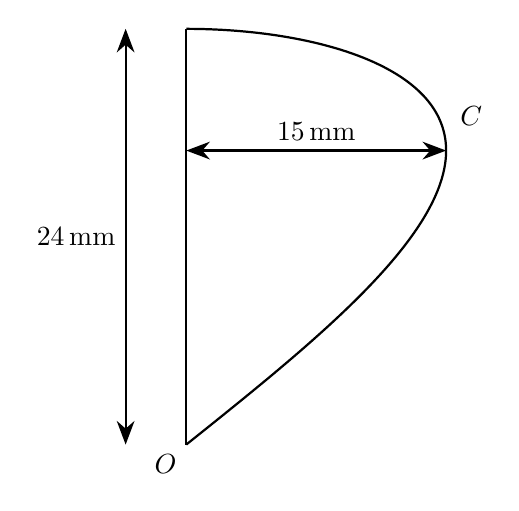
\begin{tikzpicture}[scale=1.1]
\def\a{3}
\def\b{4.8}
\pgfmathsetmacro{\ymid}{\b/sqrt(2)}

\coordinate (O) at (0,0);
\coordinate (T) at (0,\b);
\coordinate (A) at (0,\ymid);
\coordinate (W) at (\a,\ymid);
\coordinate (H1) at (-0.7,0);
\coordinate (H2) at (-0.7,\b);

\draw[thick] (O) -- (T);
\draw[thick, domain=0:90, samples=200] plot ({\a*sin(2*\x)}, {\b*sin(\x)});

\draw[{Stealth[length=3mm]}-{Stealth[length=3mm]}, thick] (H1) -- (H2) node[midway, left] {$24\,\mathrm{mm}$};
\draw[{Stealth[length=3mm]}-{Stealth[length=3mm]}, thick] (A) -- (W) node[midway, above] {$15\,\mathrm{mm}$};

\node[below left] at (O) {$O$};
\node[right] at ($(W)+(0.05,0.4)$) {$C$};
\end{tikzpicture}
\end{figure}


The diagram shows the cross-section of a decorative ornament. \\

The ornament can be modelled by rotating the region enclosed by the curve $C$ and the $y$-axis about the $y$-axis. Curve $C$ has parametric equations
\[
x = 15\sin 2\theta, \quad y = 24\sin \theta, \quad 0 \leq \theta \leq \frac{\pi}{2}
\]
where $x$ and $y$ are measured in millimetres. \\
\begin{enumerate}[label=\textbf{(\alph*)}, resume]
  \item Find the volume of the ornament. \marks{5} \\
\end{enumerate}


\end{enumerate}
\end{document}
